\section{\ref{rq:how-making-change-detection-algorithm} How to implement the change detection algorithm?} \label{sec:finding-changes}

The core of this thesis is finding changes between two versions of an application. This section sets outs how changes are found in the application. In section \ref{rq:type-visualisation-answer} the comparison result is used to merge the two models into one \textit{merge graph}.

Finding changes is handled in the \verb|Testar.ChangeDetection.Core.Algorithm| namespace.The classes used for the algorithm are visualised in figure \ref{fig:class-diagram-differences}. 

\begingroup
\captionsetup{type=figure}
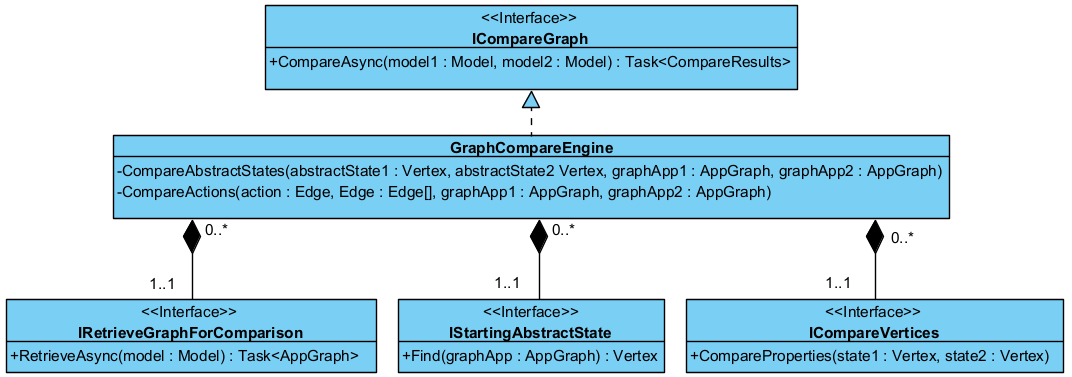
\includegraphics[scale=0.65]{images/4-UML-Differences.png}
\captionof{figure}{Class diagram, algorithm namespace (UML 2.0)}\label{fig:class-diagram-differences}
\endgroup

\subsection{The change detection algorithm} \label{sec:change-detection-algorithm}
This sub-section will explain the algorithm, starting with a high-level overview. After the high-level overview, the different interfaces in figure \ref{fig:class-diagram-differences} are explained in more detail.

The concept of \textit{corresponding states} needs to be explained to understand the algorithm. Corresponding states mean that two states, in the new and the old model, are identified as the 'same' state but can have updated GUI. There are a couple of ways to identify corresponding states. The first is by assumption, the second is inferred, and the last is by asking a third party (for example, a human input). For the developed algorithm, only the first two are used. 

Figure \ref{fig:compare-algorithm-start} gives an overview of the start of the algorithm. The \verb|GraphCompareEngine| starts with retrieving the graph data for the old and the new model. This step is indicated by step 1.1. Step 1.2 follows identical actions as 1.1 and is therefore omitted from the diagram.
\newpage

\begingroup
\captionsetup{type=figure}
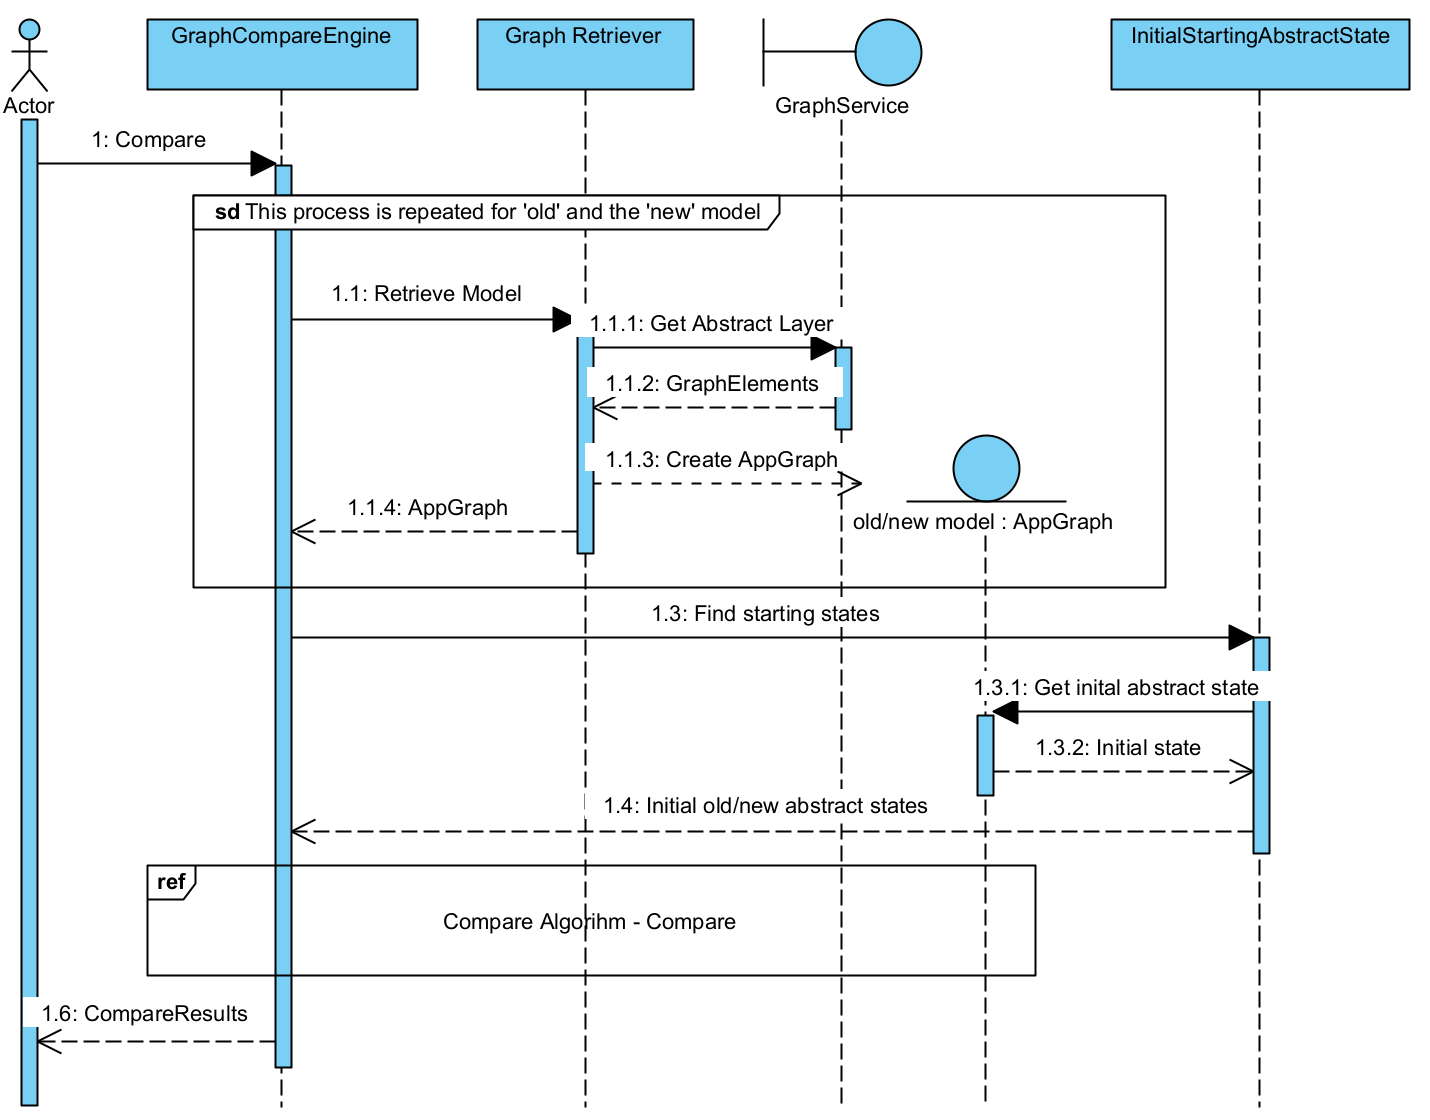
\includegraphics[scale=0.9]{content/5-Results/Images/Compare-algorithm-start.png}
\captionof{figure}{Compare Algorithm (1) - Start (UML 2.0)}\label{fig:compare-algorithm-start}
\endgroup

The next step is finding the starting states, indicated by step 1.3. Those will be the first corresponding states. The current version of the algorithm assumes that the initial states from both graphs are corresponding states. Those states could, for example, be a splash screen or a loading screen.

The flow of the algorithm continues in figure \ref{fig:compare-algorithm-compare} with 1.5. The initial states are marked as corresponding states (Step 1.5.1). The rest of the progress follows a recursive pattern between two algorithm methods, the first being \verb|CompareAbstractStates| (Step 1.5) and \verb|CompareActions| (Step 1.5.5).

The algorithm uses the abstract model to find high-level changes within the system under tests. As discussed in section \ref{abstract-model}, the concrete model contains all the information about states within the application under test, and the abstract model contains the abstracted data. Concrete states are abstracted into abstract states, and concrete actions are abstracted into abstract actions. As so, an abstract state contains one or more abstract actions, leading to another abstract state.
 
In step 1.5, the corresponding states are compared. The first step is setting the \verb|IsHandeld| variable to ensure that states are not compared twice. Then the element data of the two abstract states are compared. The comparison is done by the \verb|ICompareVertices| interface and is discussed in more detail on the sub subsection on page \pageref{sec:i-compare-vertices}.

The last step of the \verb|CompareAbstractStates| step enumerates the new model's abstract actions. For each action, the method \verb|CompareActions| (step 1.5.5) is executed, marking the action of the new model as handled. Then it looks in the corresponding abstract state for action with the same \verb|actionId|. The action id is a hashed subset of properties, as was discussed in section \ref{state-identifiers}. 

If an abstract action is found with the same \verb|actionId|, it retrieves both actions' target state. When both states are not handled, it will call the \verb|CompareAbstractStates| (Step 1.5) to make the recursive call. Both states are marked as corresponding states. Finding corresponding states by walking through the action is the second approach to finding corresponding states: inferring.

The code for the change detection algorithm is handheld by four interfaces. Each interface is discussed in more detail below, starting with the \verb|IRetrieveGraphForComparison| interface, which downloads the graph for comparison. Secondly, the \verb|IStartingAbstractState|, responsible for finding the starting states for the comparison, then the \verb|ICompareVertices| interface, which compares the element data for two given vertexes. The last interface is \verb|ICompareGraph|, which will execute the algorithm and depend on the discussed interfaces. 

In the coming sections, the various interface and associated default implementations are explained in more detail.

\textit{Note: When comparing the methods and return values presented in this thesis and the source code, one can find a discrepancy. Some return values are decorated with the} \verb|Task<..>| \textit{object and some method have the suffix} \verb|Async|. \textit{Those technical details are omitted from the thesis since they do not provide any additional value to the algorithm. When a method returns in C\#, it is an asynchronous method that can be awaited by the called. The} \verb|await| \textit{keyword will create a non-blocking call that enabled multi-threading applications \cite{asynchronous-programming}.}

\newpage

\begingroup
\captionsetup{type=figure}
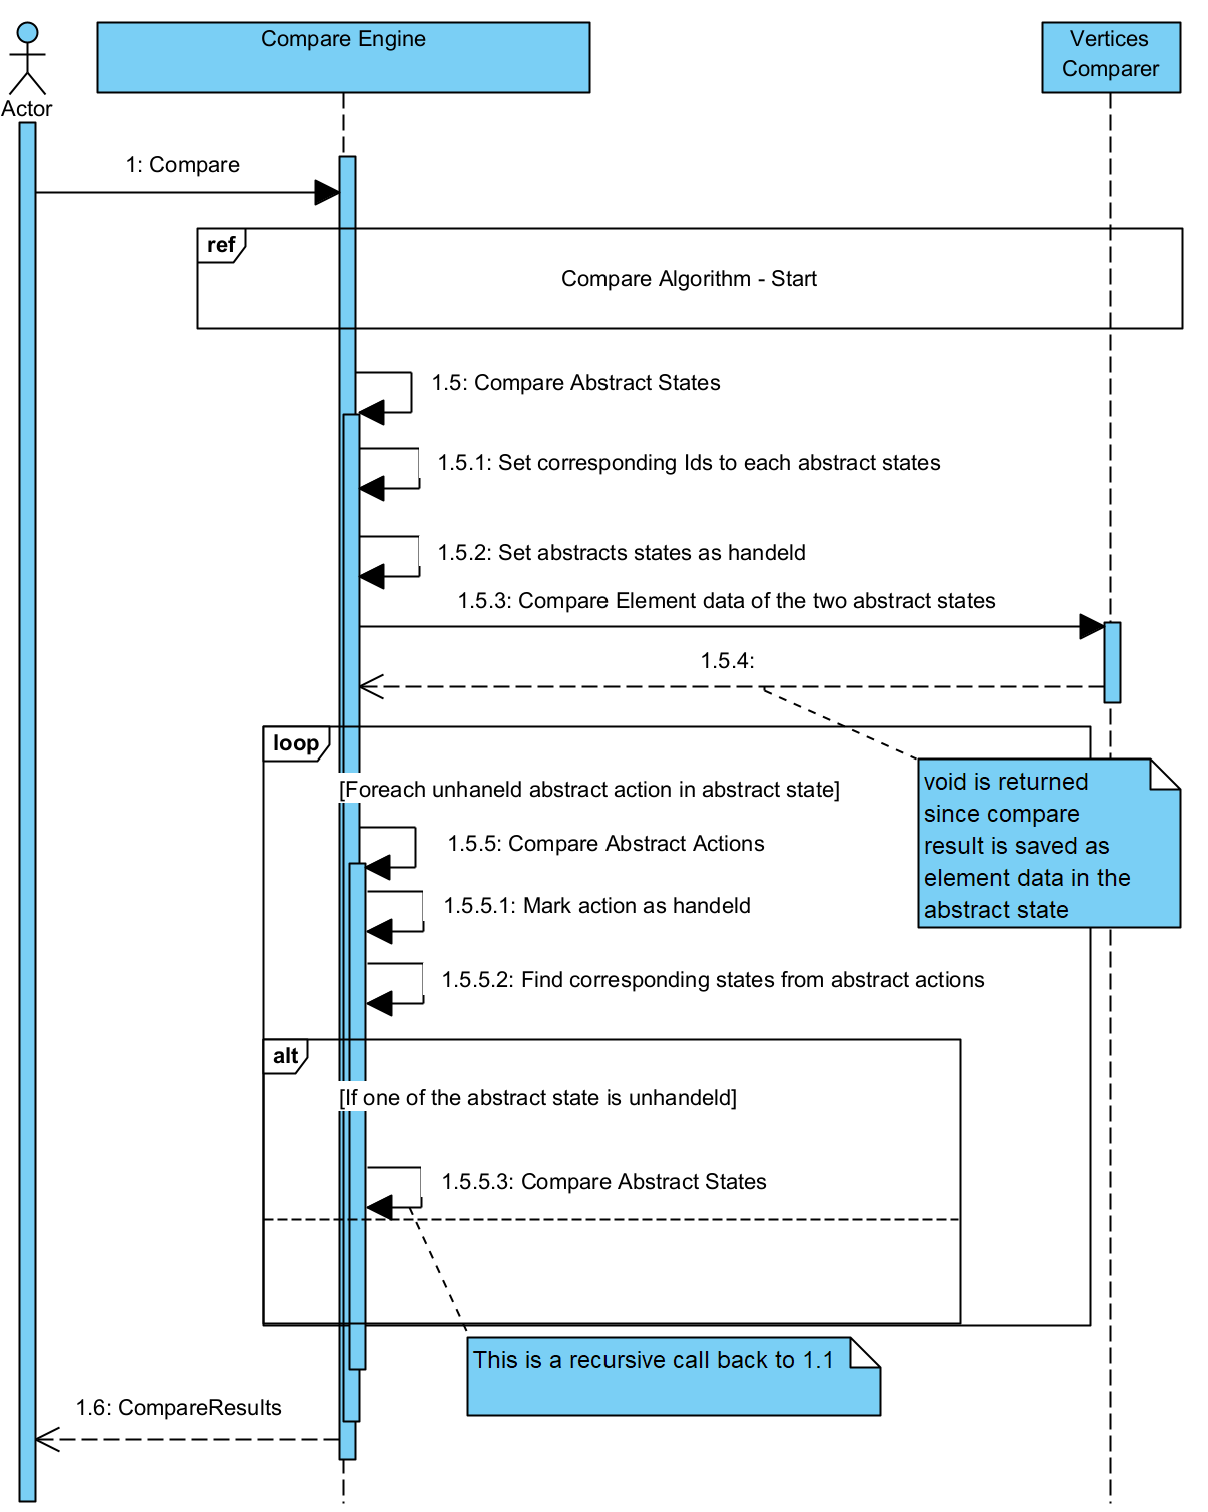
\includegraphics[scale=0.9]{content/5-Results/Images/Compare-algorithm-compare.png}
\captionof{figure}{Compare Algorithm (2) - Compare (UML 2.0)}\label{fig:compare-algorithm-compare}
\endgroup

\subsubsection{IRetrieveGraphForComparison}
The \verb|IRetrieveGraphForComparison| interface is implemented by the \verb|GraphForCompareRetriever| and is responsible for retrieving the graph data from the server. It has a dependency on the GraphService, which is an class the provided methods to retrieve the raw data from the database. 

Given a \verb|Model|, which contains the application name and version, the data from the abstract Layer, the concrete Layer and the abstract concrete connectors are retrieved. Only the data from the abstract layer is used for the comparison. The data from the concrete layer and the abstract concrete connectors are downloaded so that they can be used in the visualisation of the presentation of the graph (Discussed in more detail in \ref{rq:type-visualisation-answer}), likewise is the enrichment of the abstract actions with the description from the corresponding concrete actions.

\begingroup
\captionsetup{type=figure}
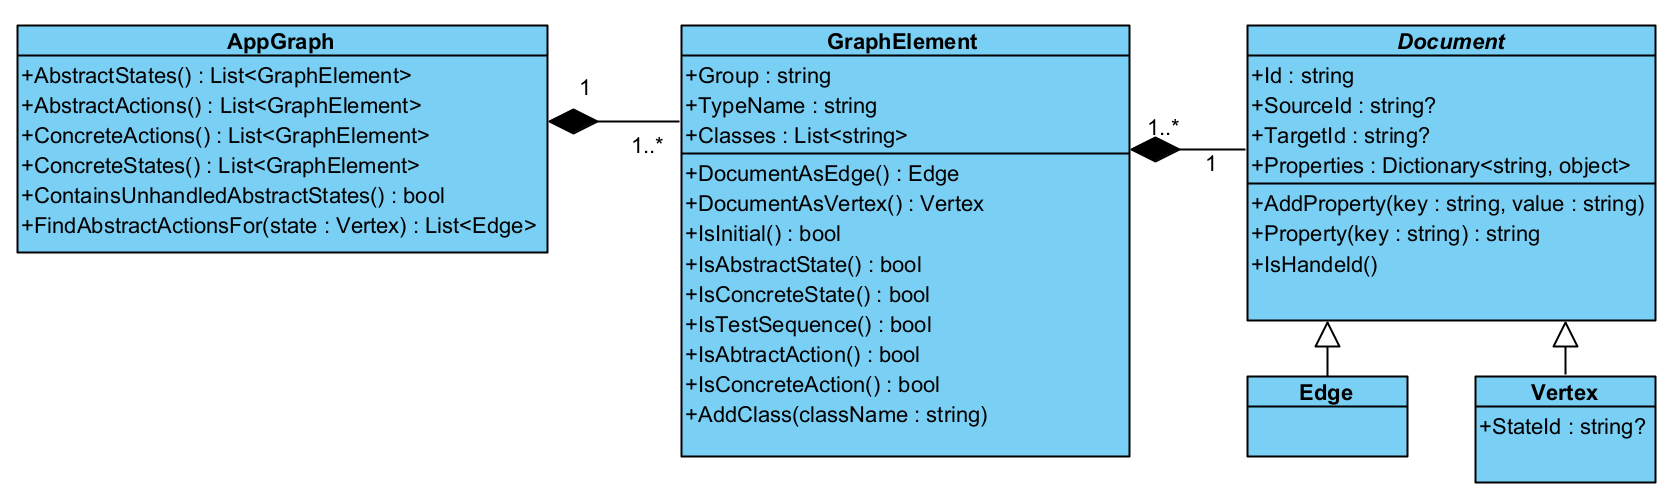
\includegraphics[scale=0.6]{images/4-UML-Models.png}
\captionof{figure}{Class diagram Graph models (UML 2.0)}\label{fig:class-diagram-models}
\endgroup

The \verb|AppGraph| class, shown in figure \ref{fig:class-diagram-models}, is wrapper around a collection of \verb|GraphElement|'s. The \verb|GraphElement| is a container of an abstract document for either a Vertex or an Edge. The abstract \verb|Document| class contains the properties from the vertex or the Edge.

Although the data for each element is located as set of properties, the classes in figure \ref{fig:class-diagram-models} contains some helper properties, e.g. \verb|IsAbstractAction| and \verb|IsConcreteState| which returns a Boolean depending on the type name. 

\subsubsection{IStartingAbstractState} \label{sec:starting-abstract-state}
The interface \verb|IStartingAbstractState| is used to locate at which abstract state the algorithm must start comparing. The default implementation is given by the \verb|InitialStartingAbstractState|. As the class name suggests, this implementation looks for the initial state. For the correct working of the algorithm, it is assumed that the initial states are corresponding states. For example, the initial states can be a splash or a loading screen.

\subsubsection{ICompareVertices} \label{sec:i-compare-vertices}
When the algorithm finds corresponding states, it needs to compare the states together. This comparison is handled by the \verb|ICompareVertices| interface. A default implementation is provided by the \verb|CompareVertices| class. In algorithm \ref{alg:comparison-corresponding-states} is explained how the inner workings of the implementation are working.  

\begin{algorithm}
    \caption{Vertex comparison}\label{alg:comparison-corresponding-states}
    \begin{algorithmic}
        \Require Element data of old model
        \Require Element data of new model
        \State $O$ = Element data of old model
        \State $N$ = Element data of new model
        \For{$p \in$ $(O \cup N)$}
            \State Mark $p$ as \textit{Added} in new model
        \EndFor
        \For{$p \in$ $(N \cup O)$}
            \State Mark $p$ as \textit{Removed} in old model
        \EndFor
        \For{$p \in$ $(O \cap N)$}
            \State $O_v$ = value of element data in old model
            \State $N_v$ = value of element data in new model
            \If{$O_v \neq N_v$}
               \State Mark element data as changed 
            \EndIf
        \EndFor
    \end{algorithmic}
\end{algorithm}

All the findings of algorithm \ref{alg:comparison-corresponding-states} are saved as element data with the prefix \verb|CD_| (for Change Detection) so that the visualisation can find them easily. Moreover, changed element data is prefixed with \verb|CD_CO_| or \verb|CD_CN_| (respectively CO standing for Changed Old value and CN for Changed New value), and new data elements are prefixed with \verb|CD_A_| (A for added) and removed data elements are prefixed with \verb|CD_R_| (R for removed).
\newpage
\subsubsection{ICompareGraph} \label{sec:compare-algorithm}
A high-level overview of the change detection algorithm is given at the start of this section (\ref{sec:change-detection-algorithm}). The algorithm is implemented in the \verb|GraphCompareEngine| class and uses the aforementioned interfaces as dependencies. The \verb|Compare| method is given 

A limitation of change detection is that the object, in this case, the old and new version of an application, needs to be similar enough to enable the detection of changes in the first place \cite{andrews2009visual}. To verify whether the similarity requirement is met, the used abstract attributes of the two versions are compared, and when different abstract attributes are used, the comparison process is cancelled \cite{stateDiff}. 